\documentclass{article}%
\usepackage[T1]{fontenc}%
\usepackage[utf8]{inputenc}%
\usepackage{lmodern}%
\usepackage{textcomp}%
\usepackage{lastpage}%
\usepackage{authblk}%
\usepackage{graphicx}%
%
\title{Imbalance between pSmad3 and Notch induces CDK inhibitors in old muscle stem cells}%
\author{Rebecca Johnson}%
\affil{Department of Biology and Biochemistry and the Centre for Regenerative Medicine, University of Bath, Bath, United Kingdom, \newline%
    Department of Pharmacy and Pharmacology and the Centre for Regenerative Medicine, University of Bath, Bath, United Kingdom}%
\date{01{-}01{-}2013}%
%
\begin{document}%
\normalsize%
\maketitle%
\section{Abstract}%
\label{sec:Abstract}%
This article was originally published on Editrix blog.\newline%
Writer April Murphy's bio profiles her three siblings, the only deceased member of the family. In honor of the one year anniversary of her passing, her message has resurfaced in her eulogy. The message refers to a genetic disease that takes the life of children and that ultimately leads to digestive ailments and even cancer.\newline%
April Murphy, a writer and physician's assistant living in Fullerton, California, was ill for the most part with the illness for nearly a decade before she was finally taken off life support last fall. She had a unique diagnosis: toxoplasmosis, a rare disease that impacts up to one in 10,000 people. The diseases is rare, and the symptoms aren't usually on the same level as colitis, kidney stones or amniotic fluid leaks, but cancer and digestive issues are more common.\newline%
Toxoplasmosis was originally treated with fecal transplants and antibiotics, but the doctors found the only cure was a rare product of gut bacteria, lysaplasm (finyanins), which is specially made for the treatment of triclosan, which is used in antibacterial alternatives. The alternative E. coli peptide is a critical component of the Food and Drug Administration's (FDA) antibacterial gel line. But lysaplasm didn't inhibit toxoplasmosis, and now the FDA is looking to prohibit this product.\newline%
Triclosan doesn't belong on the shelves of American pharmacies, yet FDA and medical experts fear it will soon be regulated by the European Union.\newline%
Lysaplasmoses form in the intestines and blood stream of immune{-}compromised patients who ingest the chemical, and among the people who do, they occur in 8{-}10 percent of all cases, according to the FDA.\newline%
Triclosan is often used as an antimicrobial substitute. In the 1970s, the FDA banned the use of the product in oral hygiene products. In 2001, the FDA authorized its use in the formulation of antimicrobial gel products.\newline%
In May, FDA proposed to end anti{-}microbial antimicrobial products's commercial development. The agency stated that antimicrobial peptides cannot change their functions even when they are taken in concentrations larger than 0.03 percent.\newline%
Tecomulus phagocytosis or toxoplasmosis is a rare genetic disease with the potential to lead to the relapse of cancer, kidney stones, urinary tract disorders and other conditions. It affects 2{-}3\% of people. Fortunately, out of those children that survive the disease, about 50\% are girls.\newline%
It wasn't easy for April Murphy to take the medical care of her one{-}year{-}old son, Jace, for a spin. Her sons were full{-}time caregivers for her elderly parents, and Jace taught Jace to use the pail of medicines. Jace would brush his teeth, get ready and wait until Jace left for school. Now he has to do every day for two entire years. It hasn't been easy for Jace's mother, and April Murphy is highly visible in her quest to protect other children from the deadly condition.

%
\subsection{Image Analysis}%
\label{subsec:ImageAnalysis}%


\begin{figure}[h!]%
\centering%
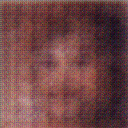
\includegraphics[width=150px]{500_fake_images/samples_5_106.png}%
\caption{A Black And White Photo Of A Vase With Flowers}%
\end{figure}

%
\end{document}